\documentclass[border=10pt]{standalone}
\usepackage{tikz}\usepackage{amsmath}\usetikzlibrary{arrows.meta}
\begin{document}
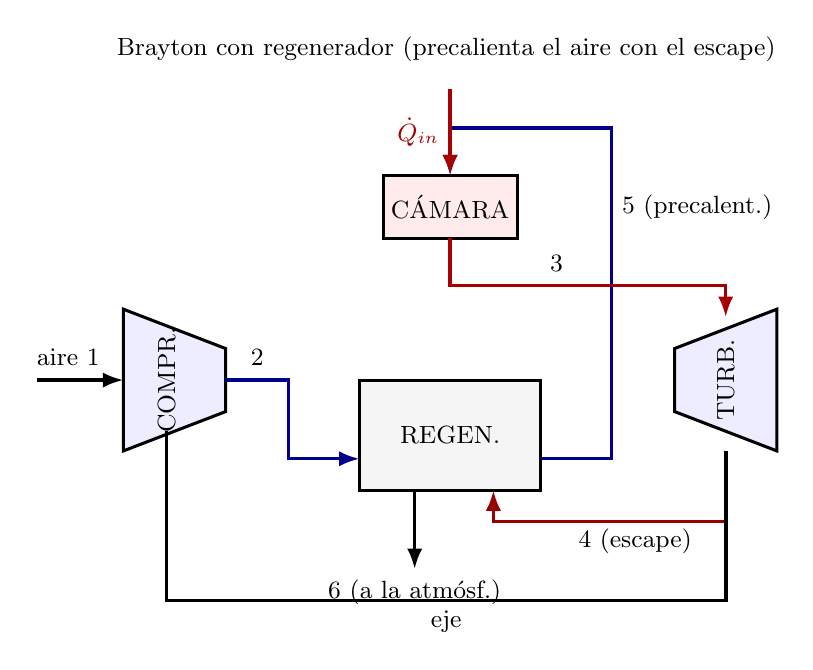
\begin{tikzpicture}[line width=1pt,>={Latex[length=2.6mm]}]
  % compresor y turbina (abajo)
  \fill[blue!7] (0,0.3)--(0,2.1)--(1.3,1.6)--(1.3,0.8)--cycle; \draw[line width=1.1pt] (0,0.3)--(0,2.1)--(1.3,1.6)--(1.3,0.8)--cycle;
  \node[rotate=90] at (0.55,1.2){\small COMPR.};
  \fill[blue!7] (7.0,0.8)--(7.0,1.6)--(8.3,2.1)--(8.3,0.3)--cycle; \draw[line width=1.1pt] (7.0,0.8)--(7.0,1.6)--(8.3,2.1)--(8.3,0.3)--cycle;
  \node[rotate=90] at (7.65,1.2){\small TURB.};
  % regenerador (centro): dos corrientes en contraflujo
  \fill[black!4] (3.0,-0.2) rectangle (5.3,1.2); \draw[line width=1.1pt] (3.0,-0.2) rectangle (5.3,1.2);
  \node[align=center] at (4.15,0.5){\small REGEN.};
  % camara combustion (arriba)
  \fill[red!8] (3.3,3.0) rectangle (5.0,3.8); \draw[line width=1.1pt] (3.3,3.0) rectangle (5.0,3.8);
  \node at (4.15,3.4){\small CÁMARA};
  % --- corriente de aire (fría) ---
  \draw[->,line width=1.2pt] (-1.1,1.2)--(0,1.2); \node[above] at (-0.7,1.25){\small aire 1};
  \draw[->,blue!55!black,line width=1.2pt] (1.3,1.2)--(2.1,1.2)--(2.1,0.2)--(3.0,0.2); \node[above] at (1.7,1.25){\small 2};
  \draw[->,blue!55!black,line width=1.2pt] (5.3,0.2)--(6.2,0.2)--(6.2,4.4)--(4.15,4.4)--(4.15,3.8); \node[right] at (6.2,3.4){\small 5 (precalent.)};
  \draw[->,red!65!black,line width=1.2pt] (4.15,3.0)--(4.15,2.4)--(7.65,2.4)--(7.65,2.0); \node[above] at (5.5,2.45){\small 3};
  % --- gases de escape (calientes) ---
  \draw[->,red!60!black,line width=1.2pt] (7.65,0.3)--(7.65,-0.6)--(4.7,-0.6)--(4.7,-0.2); \node[below] at (6.5,-0.55){\small 4 (escape)};
  \draw[->,line width=1.2pt] (3.7,-0.2)--(3.7,-1.2); \node[below] at (3.7,-1.2){\small 6 (a la atmósf.)};
  % Q_in, eje, W
  \draw[->,red!65!black,line width=1.3pt] (4.15,4.9)--(4.15,3.8) node[midway,left]{\small $\dot Q_{in}$};
  \draw[line width=1.3pt] (0.55,0.55)--(0.55,-1.6)--(7.65,-1.6)--(7.65,0.3); \node[below] at (4.1,-1.6){\small eje};
  \node at (4.1,5.4){\small Brayton con regenerador (precalienta el aire con el escape)};
\end{tikzpicture}
\end{document}
